\section{Introducción}

Aunque los sistemas satelitales han transformado el acceso a las comunicaciones en regiones de difícil conectividad terrestre, su vulnerabilidad inherente sigue representando un desafío crítico. Resulta particularmente llamativo observar cómo un único punto de fallo puede comprometer servicios esenciales para millones de usuarios, especialmente en naciones con geografías complejas y demandas crecientes de soberanía digital.

\subsection{Antecedentes del VENESAT-2}

Venezuela ha apostado históricamente por la tecnología satelital para garantizar cobertura nacional en telecomunicaciones. El VENESAT-1, también conocido como Simón Bolívar, constituyó el pilar de esta estrategia desde su lanzamiento en 2008. Sin embargo, el 13 de marzo de 2020, el satélite sufrió una falla catastrófica en sus arrays solares que lo dejó sin control, derivando en una órbita inútil y el cese total de operaciones \cite{VenesatStatus2020}. 

Este incidente no solo interrumpió servicios de televisión, telefonía e internet, sino que expuso la fragilidad de depender de un único activo en órbita geoestacionaria. Ante esta realidad, surgieron planes para el VENESAT-2 como sucesor directo, con el objetivo de restaurar y expandir capacidades. El nuevo satélite se concibe bajo exigencias más estrictas de resiliencia, incorporando desde su diseño consideraciones de redundancia que el anterior no contempló con suficiente profundidad.

\begin{table}[h]
\centering
\caption{Especificaciones principales del VENESAT-2 (proyectadas)}
\label{tab:venesat2_specs}
\begin{tabular}{ll}
\hline
\textbf{Parámetro} & \textbf{Valor} \\
\hline
Órbita & GEO (aprox. 78° W) \\
Banda principal & Ku/Ka \\
Transpondedores & >30 (estimado) \\
Vida útil diseñada & 15+ años \\
Cobertura primaria & Territorio nacional y región andina \\
\hline
\end{tabular}
\end{table}

La Tabla 1 resume las especificaciones clave que guían el presente estudio. Particularmente relevante resulta la ampliación hacia banda Ka, que promete mayor ancho de banda pero introduce complejidades adicionales en propagación bajo condiciones tropicales.

\subsection{Problemática de fallos en sistemas satelitales}

Lejos de ser un caso aislado, la experiencia del VENESAT-1 refleja una problemática más amplia en la industria. Satélites GEO enfrentan riesgos constantes: radiación, micrometeoritos, agotamiento de propelente y fallos en subsistemas críticos. En muchos casos estudiados, la ausencia de mecanismos de redundancia efectivos transforma fallos menores en interrupciones totales del servicio.

La literatura reciente tiende a destacar que arquitecturas tradicionales 1:1 ofrecen mejoras limitadas frente a escenarios de degradación progresiva o eventos correlacionados, como tormentas geomagnéticas. No obstante, cabe matizar que la implementación de redundancia no es trivial: incrementa costos, complejidad operativa y demandas de espectro. En entornos como el venezolano, donde la atenuación por lluvia representa un factor dominante, estas consideraciones adquieren peso específico.

\begin{figure}[h]
\centering
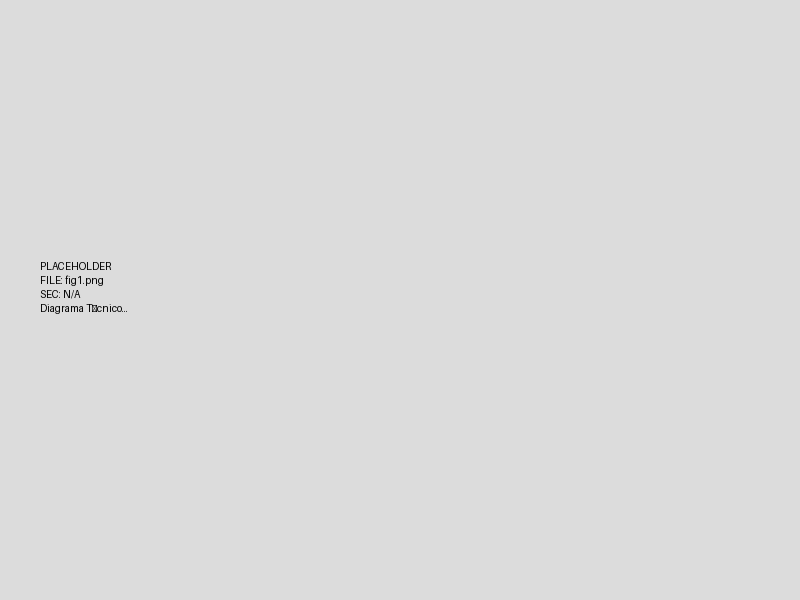
\includegraphics[width=\linewidth]{fig1.png}
\caption{Cobertura geográfica principal del VENESAT-2 sobre territorio venezolano y regiones adyacentes}
\label{fig:cobertura}
\end{figure}

La Figura 1 ilustra la huella de cobertura proyectada, destacando la necesidad de asegurar continuidad en zonas remotas de difícil acceso terrestre.

\subsection{Objetivos e hipótesis}

Uno de los desafíos persistentes que surge al analizar proyectos de esta envergadura consiste en equilibrar viabilidad técnica con restricciones operativas y presupuestarias reales. El presente estudio de factibilidad aborda precisamente esta tensión.

Los objetivos principales incluyen evaluar arquitecturas de enlace redundante (1+1 y diversidad satelital-terrestre) para el VENESAT-2, determinar su impacto en disponibilidad superior al 99.9\% y analizar implicaciones operativas bajo condiciones tropicales. Se examinan balance de enlace, modelos de propagación ITU-R y análisis FMEA de confiabilidad.

Se plantea como hipótesis central que una implementación redundante bien diseñada no solo mitiga los riesgos observados en VENESAT-1, sino que genera márgenes operativos suficientes para justificar la inversión en el contexto venezolano. Investigaciones recientes sobre redundancia en sistemas satelitales parecen sugerir que configuraciones híbridas ofrecen el mejor compromiso entre resiliencia y eficiencia \cite{SatCommRedundancy2024}.

Este trabajo delimita su alcance a la factibilidad técnica y operativa, dejando para fases posteriores el análisis económico detallado y la implementación física. Los hallazgos que aquí se presenten pretenden servir como base rigurosa para decisiones estratégicas orientadas a fortalecer la infraestructura satelital del país.